\documentclass[12pt]{article}


\usepackage{amssymb}
\usepackage{amsmath}
\usepackage{fullpage}
\usepackage{epsfig}
\usepackage{epstopdf, xcolor, hyperref}
\everymath{\displaystyle}
\usepackage{enumerate}

\newif\ifans

\anstrue

\begin{document}

\begin{center}
\underline{\LARGE{Cross Product}}
\end{center}

\noindent SUGGESTED REFERENCE MATERIAL:

\bigskip

\noindent As you work through the problems listed below, you should reference Chapter 11.4 of the recommended textbook (or the equivalent chapter in your alternative textbook/online resource) and your lecture notes.

\bigskip

\noindent EXPECTED SKILLS:

\begin{itemize}

\item Know how to compute the cross product of two vectors in $\mathbb{R}^3$. 

\item Be able to use a cross product to find a vector perpendicular to two given vectors.

\item Know how to use a cross product to find areas of parallelograms and triangles.

\item Be able to use a cross product together with a dot product to compute volumes of parallelepipeds.

\end{itemize}

\noindent PRACTICE PROBLEMS:

\medskip

\begin{enumerate}

\item For each of the following, compute $\overrightarrow{u}\times\overrightarrow{v}$ and verify that it is orthogonal to both $\overrightarrow{u}$ and $\overrightarrow{v}$.

\begin{enumerate}

\item $\overrightarrow{u}=\langle 3,-4,1 \rangle$; $\overrightarrow{v}=\langle 2,-2,3 \rangle$

\ifans{\fbox{$\langle -10,-7,2\rangle$}} \fi

\item $\overrightarrow{u}=\langle 2,-2,6 \rangle$; $\overrightarrow{v}=\langle -1,2,-1 \rangle$

\ifans{\fbox{$\langle -10,-4,2\rangle$}} \fi

\item ${\bf u}=2{\bf i}+3{\bf k}$; ${\bf v}={\bf i}-{\bf j}$

\ifans{\fbox{$\langle 3,3,-2\rangle$}} \fi

\end{enumerate}

\item \begin{enumerate}

\item Using appropriate properties of the cross product ({\bf Not Determinants}), compute $({\bf i}-{\bf j})\times({\bf j}-{\bf i})$.

\ifans{\fbox{${\bf 0}$; Detailed Solution: \textcolor{blue}{\href{http://www.math.drexel.edu/classes/Calculus/resources/Math200HW/Solutions/04_200_Cross_Product_02.pdf}{Here}} }} \fi

\item Verify that your answer to part (a) is correct by using determinants.

\ifans{\fbox{${\bf 0}$; Detailed Solution: \textcolor{blue}{\href{http://www.math.drexel.edu/classes/Calculus/resources/Math200HW/Solutions/04_200_Cross_Product_02.pdf}{Here}} }} \fi

\end{enumerate}

\item Compute two unit vectors which are normal to the plane which is determined by the points $A(1,2,3)$, $B(6,4,7)$, and $C(1,5,2)$.

\ifans{\fbox{$\overrightarrow{u_{1,2}}=\pm\frac{1}{\sqrt{446}}\langle -14,5,15 \rangle$}} \fi

\item Compute the area of the triangle with vertices $A(1,2,3)$, $B(6,4,7)$, and $C(1,5,2)$.

\ifans{\fbox{$\frac{1}{2}\sqrt{446}$}} \fi

\item Compute $\|{\bf u} \times {\bf v}\|$ if $\|{\bf u}\|=2$, $\|{\bf v}\|=5$, and the angle between ${\bf u}$ and ${\bf v}$ is $30^{\circ}$.

\ifans{\fbox{5}} \fi

\item The following questions deal with finding the distance from a point to a line:

\begin{enumerate}

\item Given three points $A$, $B$, and $P$ in 3-space as shown in the picture below, explain how you could use the cross product to calculate the distance, $d$, between the point $P$ and the line which contains $A$ and $B$.  

\begin{center}
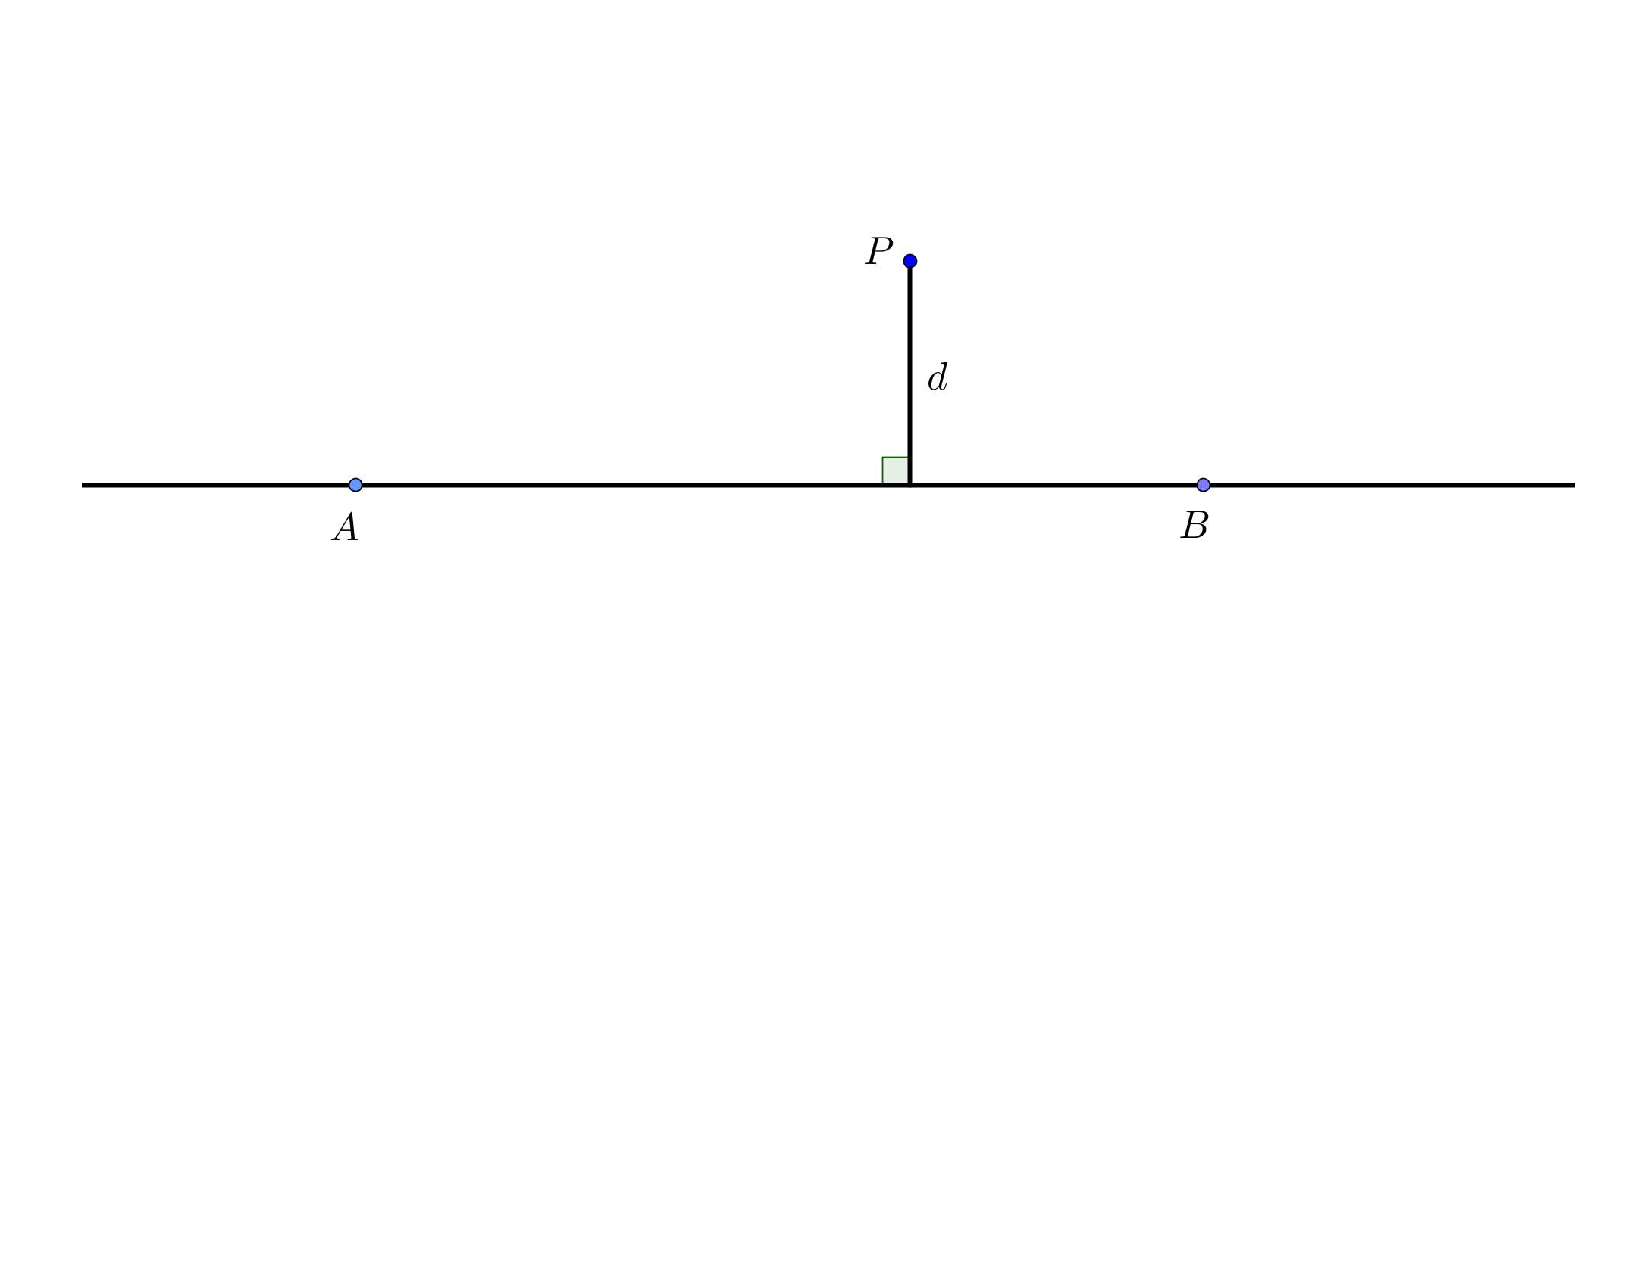
\includegraphics[scale=0.5]{length.pdf}
\end{center}

(Hint: Consider the vectors ${\bf AP}$ and ${\bf AB}$)

\ifans{\fbox{\parbox{1\linewidth}{Let $\theta$ be the angle between ${\bf AP}$ and ${\bf AB}$.  Then:
\begin{align*}
d&=\|{\bf AP}\|\sin{\theta}\\
&=\frac{\|{\bf AP}\|\|{\bf AB}\|\sin{\theta}}{\|{\bf AB}\|}\\
&=\frac{\|{\bf AP}\times{\bf AB}\|}{\|{\bf AB}\|}
\end{align*}
}}} \fi

\item Use your method from part (a) to compute the distance from the point $P(5,3,0)$ to the line containing $A(1,0,1)$ and $B(2,3,1)$.  Verify your answer with HW 11.3 \#10(b).

\ifans{\fbox{$d=\sqrt{\frac{91}{10}}$}} \fi

\end{enumerate}

\item Consider the parallelepiped with adjacent edges $\overrightarrow{u}=\langle1,2,3\rangle$, $\overrightarrow{v}=\langle3,4,0\rangle$, and $\overrightarrow{w}=\langle-1,3,-2\rangle$.

\begin{enumerate}

\item Compute the volume of the parallelepiped.

\ifans{\fbox{43; Detailed Solution: \textcolor{blue}{\href{http://www.math.drexel.edu/classes/Calculus/resources/Math200HW/Solutions/04_200_Cross_Product_07.pdf}{Here}}}} \fi

\item Determine the area of the face determined by $\overrightarrow{v}$ and $\overrightarrow{w}$.

\ifans{\fbox{$\sqrt{269}$; Detailed Solution: \textcolor{blue}{\href{http://www.math.drexel.edu/classes/Calculus/resources/Math200HW/Solutions/04_200_Cross_Product_07.pdf}{Here}}}} \fi

\item Compute the angle between $\overrightarrow{u}$ and the plane containing the face determined by $\overrightarrow{v}$ and $\overrightarrow{w}$.

\ifans{\fbox{$\frac{\pi}{2}-\cos^{-1}\left(\frac{43}{\sqrt{14}\sqrt{269}}\right)$; Detailed Solution: \textcolor{blue}{\href{http://www.math.drexel.edu/classes/Calculus/resources/Math200HW/Solutions/04_200_Cross_Product_07.pdf}{Here}}}} \fi

\end{enumerate}

\item {\bf Multiple Choice:} Suppose ${\bf u}$ and ${\bf v}$ are non-zero vectors in $\mathbb{R}^3$ and that ${\bf u}\cdot{\bf v}=\|{\bf u}\times{\bf v}\|$, which of the following is the angle between ${\bf u}$ and ${\bf v}$?

\begin{enumerate}

\item 0

\item $\frac{\pi}{6}$

\item $\frac{\pi}{4}$

\item $\frac{\pi}{3}$

\item $\frac{\pi}{2}$

\end{enumerate}

\ifans{\fbox{c}} \fi

\item {\bf True or False:}  Mark each of the following as either true or false. If the statement is false, explain why or provide a counterexample.

\begin{enumerate}

\item The cross product of two vectors in $\mathbb{R}^3$ is \underline{anti-commutative}; i.e., ${\bf v}\times{\bf w}=-({\bf w}\times{\bf v})$.

\ifans{\fbox{True}} \fi

\item ${\bf i}\times{\bf k}={\bf j}$.

\ifans{\fbox{False; ${\bf i}\times{\bf k}=-{\bf j}$}} \fi

\item For any vectors ${\bf u}$ and ${\bf v}$ in $\mathbb{R}^3$, $\|{\bf u}\times{\bf v}\|=\|{\bf v}\times{\bf u}\|$.

\ifans{\fbox{True}} \fi

\item If ${\bf u}\times{\bf v}={\bf 0}$, then either ${\bf u}={\bf 0}$ or ${\bf v}={\bf 0}$.

\ifans{\fbox{False; If ${\bf u}$ is parallel to ${\bf v}$, then ${\bf u}\times{\bf v}={\bf 0}$.}} \fi

\item If ${\bf u}\cdot {\bf v}=0$ and ${\bf u}\times{\bf v}={\bf 0}$, then either ${\bf u}={\bf 0}$ or ${\bf v}={\bf 0}$.

\ifans{\fbox{True}} \fi

\end{enumerate}

\end{enumerate}

\end{document}